\chapter{Conclusion}
\label{chapter:conclusion}

\section{Summary}
\label{sec:conclusion_summary}

This dissertation studied how machine learning can organize neural and visual observations into representations that support cognition-related prediction, semantic decoding, and interaction. Its four core chapters moved from neural structure to semantic content, from visual semantics to action representations, and finally to physical action.

\hybrid{} learned high-order relationships among brain regions as weighted hyperedges. Its multi-head drop-bottleneck made it possible to learn informative structures from a large space of possible region combinations while limiting irrelevant information. The experiments showed that incorporating these learned high-order relationships improved the model's prediction performance.

\mindllm{} extended the focus to semantic content associated with brain activity. Its subject-agnostic encoder used voxel locations and brain-region information to organize irregular sets of fMRI measurements. Brain Instruction Tuning connected those measurements to existing annotations through shared stimulus images. Together, the encoder and instruction-tuning procedure supported subject-generalizable semantic decoding across perception, language, and knowledge-related tasks.

\mwm{} connected semantics to action by using visual consequences to supervise motor representation learning. A world model predicted future visual features conditioned on an EEG-derived latent action, so the semantics of the observed consequences provided a training signal for the EEG encoder without action annotations. The Lateralization-Aware Transformer incorporated the left--right organization of motor EEG into this learning process. The resulting mind model transferred to motor decoding, while the retained world model supported future prediction through an action interface evaluated with independently measured IMU signals.

Following the study of action-intention decoding in \mwm{}, \dysta{} investigated how robotic policies can translate human intentions into effective and efficient task execution. Its separation of temporally persistent and dynamic visual information allowed a robotic policy to use observation history while reusing computation. Multi-frame experiments evaluated the value of memory, and inference measurements assessed the savings from static-token reuse and learned cache refresh. This work demonstrated how modeling temporally persistent structure can support both task completion and computational efficiency.

These studies address successive questions about connecting mind and world: how to identify useful neural priors and incorporate them to improve predictive performance, how to develop subject-generalizable semantic decoding, how to learn action representations through the semantics of visual consequences, and how embodied agents can realize users' action intentions effectively and efficiently. Together, these contributions connect the study of brain signals, semantics, and action to the broader goal of translating human intentions into effective interaction with the physical world.

\section{Future Directions}
\label{sec:future_directions}

% Future-work scope follows the final two research slides of
% deck/dissertationv3.pptx (slides 50--51 in presentation order).
The next direction extends the reading of neural activity toward writing through stimulation. Decoding estimates aspects of a current brain state; choosing an intervention also requires predicting how that state may change. A brain world model could provide these predictions, and a control policy could use them to select interventions toward a desired outcome. New measurements would then update the inferred state and inform the next decision. This direction involves two connected research problems: learning a model of brain dynamics and using that model for closed-loop intervention.

\subsection{Multimodal Brain World Models}
\label{sec:future_multimodal_brain_models}

A multimodal brain world model would connect fMRI, EEG, MEG, and functional ultrasound through a shared latent representation. Modality-specific encoders would map available recordings into that representation, and modality-specific decoders would map predicted states back to the corresponding observation spaces. The aim is to learn a representation that can be accessed through different recording techniques and shared across subjects. Differences in temporal resolution, spatial coverage, and individual responses make this shared representation a central modeling challenge.

A transition model would predict subsequent latent brain states, either without an external intervention or conditioned on a specified stimulus or stimulation. After an initial observation, the model could roll forward without receiving new measurements, generating candidate neural trajectories. This would give the model two related roles: a foundation model for representing neural recordings and a simulator for comparing possible interventions. Figure~\ref{fig:future_multimodal_brain_world_model} illustrates the proposed architecture.

The future prediction component of \mwm{} offers a starting point for this formulation. In \mwm{}, predicting external visual changes provides supervision for action representations learned from EEG. Here, an external intervention would condition predictions of changes in the brain itself. Establishing this capability requires evaluating responses to interventions and testing whether predictions remain reliable across individuals and over longer trajectories. 
\begin{figure}[htbp]
    \centering
    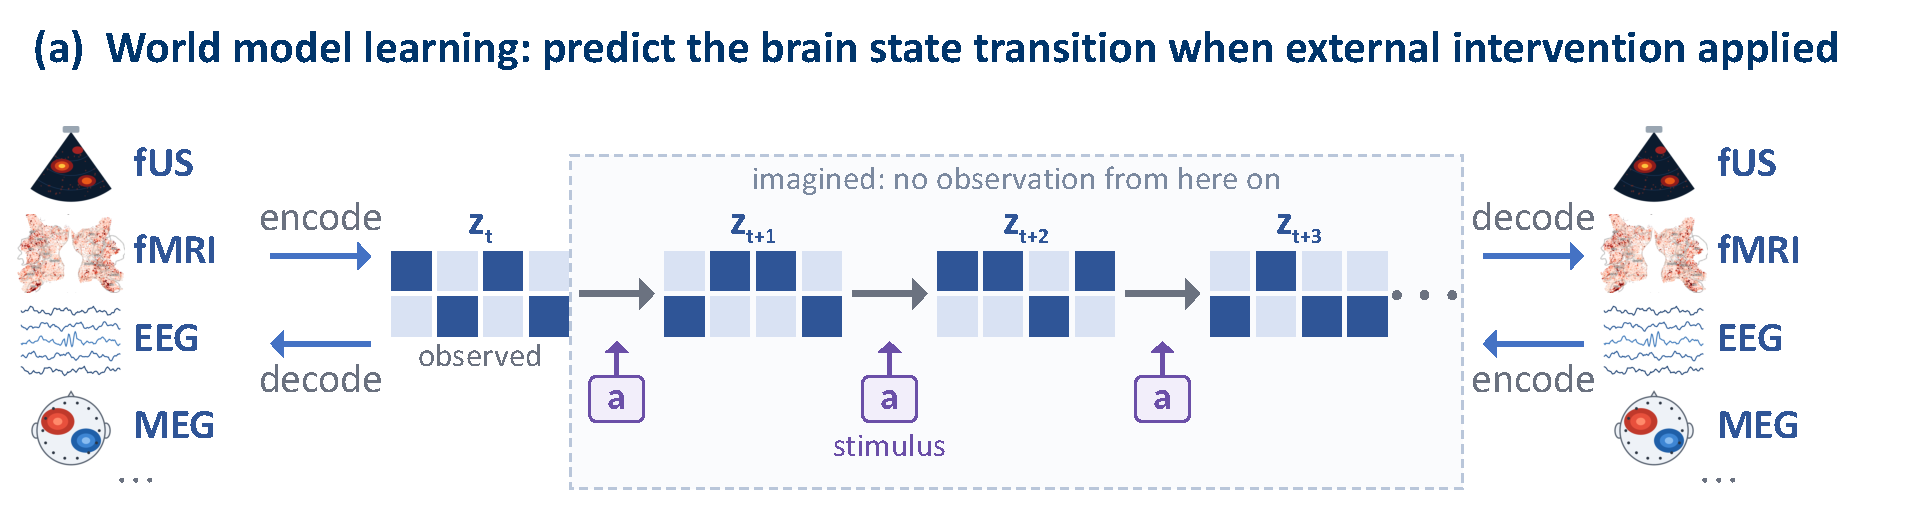
\includegraphics[width=\linewidth]{figures/future_directions/multimodal_brain_world_model.pdf}
    \caption[Proposed multimodal brain world model]{Proposed multimodal brain world model. Modality-specific encoders and decoders connect neural recordings through a shared latent state. A transition model predicts subsequent states conditioned on stimuli or stimulation and can roll forward without new observations. Learning predictions that transfer across subjects and remain valid under interventions is a research objective.}
    \label{fig:future_multimodal_brain_world_model}
\end{figure}

\subsection{Closed-Loop Intervention through Predicted Brain Dynamics}
\label{sec:future_brain_intervention}

A brain world model would provide a setting for learning an intervention policy through predicted neural trajectories. Following the Dreamer approach~\citep{hafner2025mastering}, an actor would propose an intervention and a critic would estimate its long-term value from a brain-derived latent or recurrent state. The world model would generate imagined trajectories for actor--critic training. Neural decoding would supply task-relevant feedback, connecting the learning objective to the brain state that the intervention is intended to influence. Figure~\ref{fig:future_brain_closed_loop} illustrates actor--critic learning and a prospective closed-loop application.

A prospective application is closed-loop transcranial focused ultrasound for chronic pain. A decoder would estimate a pain-related state from neural recordings and provide feedback for learning an intervention policy. The policy would select a stimulation setting with the goal of reducing pain, the brain world model would predict the response, and subsequent recordings would update the state estimate after stimulation.

\begin{figure}[htbp]
    \centering
    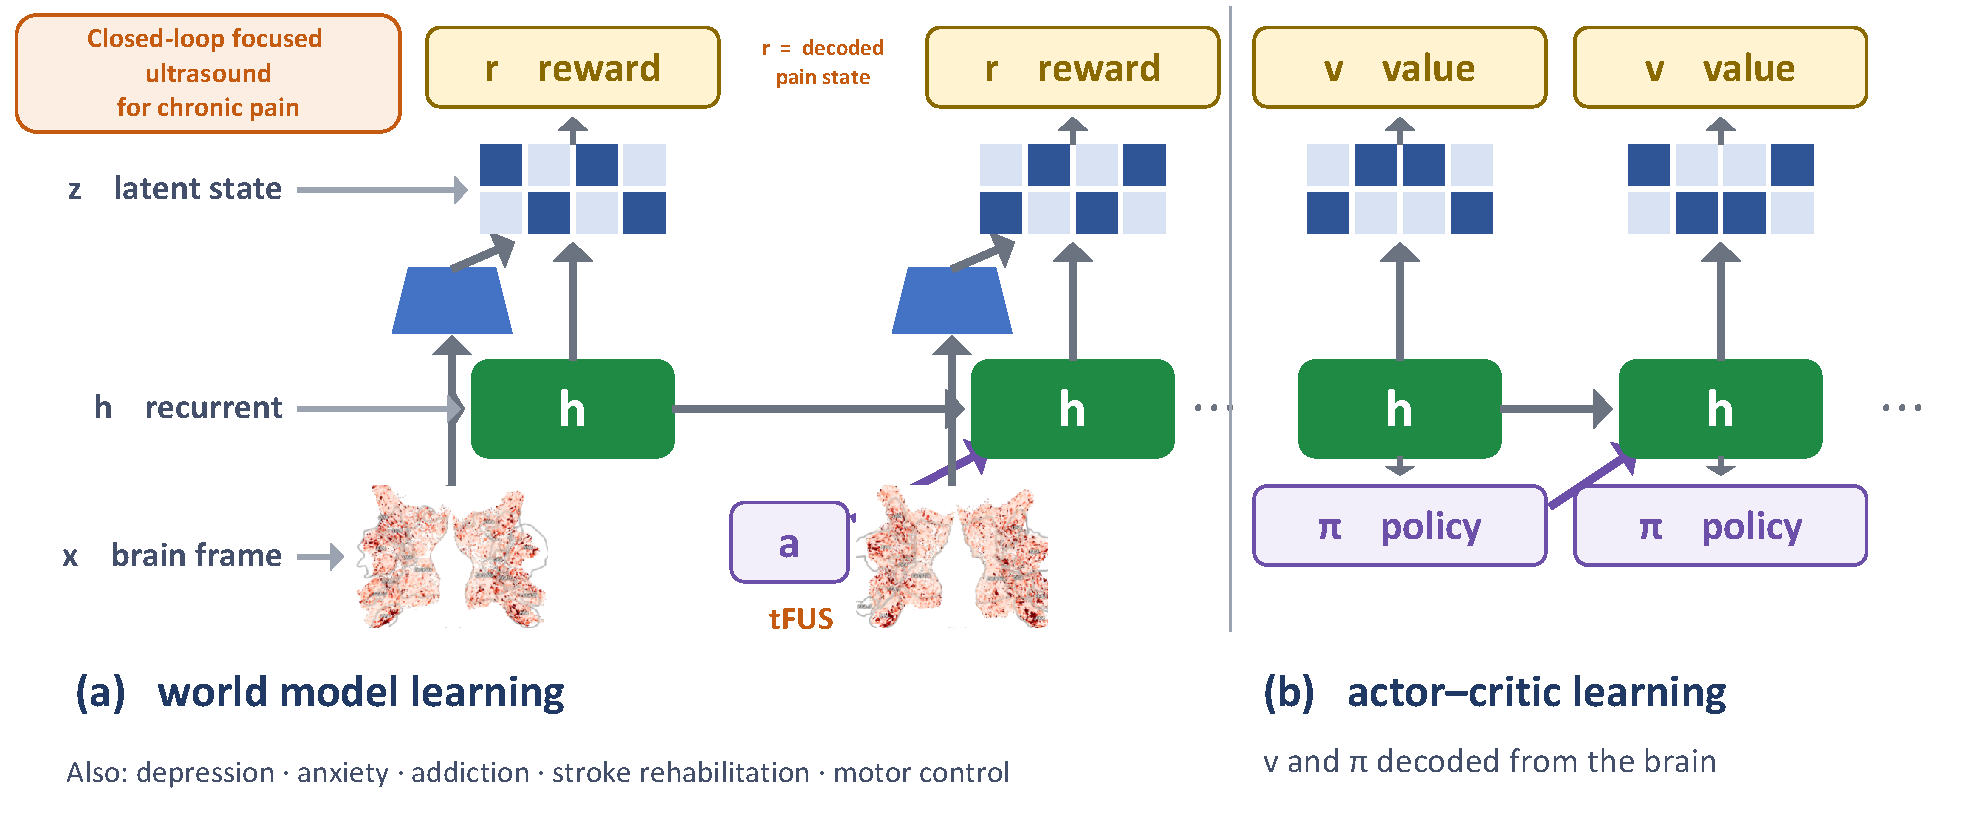
\includegraphics[width=\linewidth]{figures/future_directions/brain_closed_loop.pdf}
    \caption[Proposed closed-loop intervention through a brain world model]{Proposed closed-loop intervention through a brain world model. (a) A brain-derived state $s_t=(h_t,z_t)$, with recurrent state $h_t$ and latent state $z_t$, supplies the actor $\pi$ and value critic $v$. The intervention $a_t$ conditions imagined transitions for policy learning, following the Dreamer framework~\citep{hafner2025mastering}. (b) In the prospective chronic-pain application, the learned policy selects focused-ultrasound stimulation (tFUS), and new recordings update the state estimate. Decoded pain-related feedback $r_t$ informs policy learning.}
    \label{fig:future_brain_closed_loop}
\end{figure}

The same modeling questions could motivate future studies of depression, anxiety, addiction, and stroke rehabilitation, with objectives and validation specific to each setting. The immediate methodological goal is to connect neural state estimation, prediction under intervention, and policy learning in a loop whose predictions can be checked against new measurements. This would extend the dissertation's study of representations toward models that guide how neural states are influenced over time.
